\lhead{\begin{tikzpicture}[remember picture, overlay]
    \node [anchor=100,inner sep=0] (imagenIZQUIERDA) at (current page header area.north){
\includegraphics[width=18cm]{img/Encabezado.PNG}};
    \end{tikzpicture}}
    \rhead{Ángeles-Hurtado}
    \rfoot{\begin{tikzpicture}[remember picture, overlay]
    \node [anchor=140,inner sep=0] (imagenDERECHA) at (current page footer area.south){
\includegraphics[width=18cm]{img/Foot.PNG}};
    \end{tikzpicture}}
    %----------------------------------------------------------------------------------------
    \lfoot{ \thepage}
    % \renewcommand{\labelenumi}{\alph{enumi}.)} 
    %----------------------------------------------------------------------------------------
    %----------------------------------------------------------------------------------------
    %	TITLE SECTION
    %----------------------------------------------------------------------------------------
    
    \setlength{\droptitle}{-5\baselineskip} % Move the title up
    \title{\textbf{Estudio de tiempos y movimientos en el ensamble de un circuito electrónico utilizando diferentes métodos para su optimización }} % Article title
    
     \author{ 
     \textsc{Nieves Jimenez Ana Sofia/s}\\ 
    %  Afiliación:
     \texttt{ Instituto Tecnológico de Quéretaro } \\ 
     \texttt{Tecnológico Nacional de México } \\ 
     \texttt{Quéretaro,México}\\ 
     \texttt{} 
     \and 
     \textsc{Ángeles-Hurtado, Luis Alberto}\\ 
    %  Afiliación:
     \texttt{ Instituto Tecnológico de Querétaro } \\ 
     \texttt{ Tecnológico Nacional de México } \\ 
     \texttt{Querétaro, México}\\ 
     \texttt{alb3rt0.ah@gmail.com} 
    }
    
    
    %----------------------------------------------------------------------------------------
    
    % \begin{document}
    
    % Print the title
    \maketitle
    \thispagestyle{fancy}
    
    %----------------------------------------------------------------------------------------
    %	ARTICLE CONTENTS
    %----------------------------------------------------------------------------------------
    
    % \section*{Resumen}
    % \textit{Palabras clave:}
    % El resumen (ancho de página) deberá contener entre 100 y 200 palabras tipo Adobe Devangari 11 puntos.
    
    \begin{abstract}
    \noindent 
    El resumen (ancho de página) deberá contener entre 100 y 200 palabras tipo Adobe Devangari 11 puntos.
    
    \end{abstract}
    % 
    % 
    \textbf{\textit{Palabras clave}}: {First keyword should be the corresponding to the research area according with the authors guide. Maximum of 6 keywords.}
    % \keywords{First keyword should be the corresponding to the research area according with the authors guide. Maximum of 6 keywords.}
    
    \section{Introducción}
    
    El estudio de tiempos y movimientos implica analizar los métodos, materiales, herramientas e instalaciones utilizados o que se prevé utilizar en la ejecución de un trabajo. Este análisis tiene como objetivo describir académicamente cómo un estudiante promedio de cuarto semestre de ingeniería industrial puede adquirir las habilidades necesarias para desarrollar un trabajo desde cero mediante la implementación del estudio de tiempos y movimientos.\cite{carlos2016ingenieria}
    Para llevar a cabo este estudio, se realizará un ensamble que combinará diversas partes y elementos para crear un circuito electrónico. Considerando todos los factores se determinará , seleccionará y ajustarán los componentes necesarios para optimizar el ensamble, calculando el tiempo de ciclo, el tiempo estándar y desarrollando diferentes métodos para mejorar este proceso.
    Ahora al mencionar un circuito electrónico lo definiremos como aquel sistema compuesto por uno o más conductores, que pueden ser vistos como las direcciones que puede seguir una corriente eléctrica. En este proyecto utilizaremos un convertidor de corriente alterna a corriente directa. Cabe mencionar que tal circuito electrónico puede estar formado por diversos componentes pasivos o activos, por lo que están diseñados para cumplir alguna función específica.
    Claro en esta práctica ocuparemos una optimización que es comprendida como una búsqueda de la mejor manera de realizar una actividad. En este caso, nos referimos a optimizar el tiempo que se refiere a reducir tiempos improductivos y aumentar la eficiencia del proceso.
    Para realizar lo planteado anteriormente; utilizaré diversas herramientas, como lo es el método de tiempos predeterminados. Este consiste en reglas o procedimientos que permiten determinar de antemano la secuencia de eventos necesarios para realizar una tarea, facilitando la planeación y estandarización de los procesos. 
    Finalmente el objetivo general de este proyecto es el poder  adquirir competencias clave para el análisis y la mejora continua de procesos, para a futuro poder  enfrentar desafíos en entornos industriales reales y con esto desarrollar habilidades prácticas y teóricas en el área de la ingeniería de producción, así como en la mejora de productos y la gestión de calidad. A través de la aplicación de métodos de optimización y el uso de herramientas de tiempos predeterminados para la mejora de procesos industriales.
    %\end{itemize}
    % 
    % 
    \section{Justificación}
    
    \begin{itemize}
    \item En la actualidad, el análisis detallado de los tiempos y movimientos en el ensamble de circuitos electrónicos permite identificar áreas de ineficiencia y desperdicio de recursos, lo que se traduce en una reducción de costos y un aumento de la productividad.
    Además, en un mundo donde la tecnología avanza rápidamente, la capacidad de adaptarse y mejorar constantemente es esencial para mantenerse relevante. Mediante el uso de metodologías como los therbligs, las empresas pueden realizar ajustes precisos en sus procesos de ensamble para integrar nuevas tecnologías y responder rápidamente a las demandas cambiantes del mercado.\cite{niebel1980ingenieria}
    A nivel local o nacional, la implementación de técnicas de estudio de tiempos y movimientos en el ensamble de circuitos electrónicos puede tener un impacto significativo en la economía y la competitividad de las empresas del sector. 
    \end{itemize}
    % 
    % 
    \section{Descripción del problema}
    \begin{itemize}
        \item Un problema común en el estudio de tiempos y movimientos en el ensamble de un circuito electrónico es la identificación de movimientos innecesarios o ineficientes que afectan la productividad y la calidad del producto final. Por ejemplo, uno de los problemas que puede surgir es la falta de estandarización en el proceso de ensamble, lo que lleva a variaciones en los tiempos de ciclo y en la calidad de los productos ensamblados.
    En un entorno de producción de circuitos electrónicos, donde se ensamblan múltiples componentes en un espacio reducido, los trabajadores pueden enfrentar dificultades para acceder a los materiales y herramientas necesarios, lo que resulta en movimientos adicionales y tiempos de espera. Esto puede llevar a una disminución en la eficiencia y a un aumento en los tiempos de ciclo, lo que afecta la capacidad de la empresa para cumplir con los plazos de entrega y satisfacer las demandas del mercado.
    Además, la falta de ergonomía en el diseño de estaciones de trabajo y herramientas puede resultar en movimientos repetitivos o posturas incómodas para los trabajadores, lo que aumenta el riesgo de lesiones y fatiga laboral. Esto no solo afecta la salud y seguridad de los empleados, sino que también puede afectar la calidad del trabajo realizado y la eficiencia del proceso de ensamble en su conjunto.
    Otro problema común es la falta de capacitación adecuada para los trabajadores en cuanto a las mejores prácticas de ensamble y el uso eficiente de herramientas y equipos. Esto puede resultar en variaciones en los tiempos de ciclo y en la calidad de los productos ensamblados, así como en un aumento en los errores y retrabajos.
    En resumen, un problema importante en el estudio de tiempos y movimientos en el ensamble de circuitos electrónicos es la identificación y corrección de movimientos innecesarios, ineficientes o ergonómicamente desfavorables que afectan la productividad, la calidad y la seguridad en el lugar de trabajo. Resolver estos problemas requiere un enfoque sistemático que incluya la estandarización de procesos, el diseño ergonómico de estaciones de trabajo, la capacitación adecuada para los trabajadores y la implementación de mejoras continuas en el proceso de ensamble.
    \end{itemize}
    
    \textbf{*La incógnita científica es el elemento cuya solución incrementa el conocimiento científico.}
    % 
    % 
    \section{Fundamentación teórica}
    
    \begin{itemize}
        \item 
    El problema identificado anteriormente se manifiesta en diversas áreas del proceso de ensamble. Por un lado, la falta de estandarización en los métodos de trabajo puede dar lugar a variaciones en los tiempos de ciclo y en la calidad de los productos ensamblados. Esta falta de consistencia puede deberse a la falta de procedimientos claros, a la improvisación por parte de los trabajadores o a la ausencia de herramientas y equipos estandarizados.
    Además, la ergonomía juega un papel crucial en el proceso de ensamble. Las estaciones de trabajo mal diseñadas o las herramientas inadecuadas pueden resultar en movimientos repetitivos, posturas incómodas y riesgos de lesiones para los trabajadores. Estos problemas no solo afectan la salud y seguridad de los empleados, sino que también pueden afectar la eficiencia y la calidad del trabajo realizado.
    En cuanto a las metodologías utilizadas para abordar estos problemas, es importante considerar una variedad de enfoques. El mapeo de procesos es una herramienta útil para visualizar y comprender el flujo de trabajo en el proceso de ensamble, identificando áreas de redundancia o ineficiencia. La observación directa y el cronometraje continuo permiten registrar y analizar los movimientos y tiempos de trabajo de manera precisa. El análisis de micro movimientos descompone las actividades en acciones más pequeñas y observables, facilitando la identificación de movimientos innecesarios o ineficientes.\cite{book}
    
    \end{itemize}
    % 
    % 
    \section{Hipótesis}
    
    \begin{itemize}
        \item Un estudio de tiempos preciso y bien realizado en un entorno laboral puede mejorar la eficiencia operativa y la productividad de la organización al identificar y eliminar actividades redundantes, optimizar los procesos de trabajo y asignar recursos de manera más efectiva.
    
    Esto sugiere que el análisis sistemático de las actividades estudiantiles y el tiempo dedicado a cada una puede proporcionar información valiosa para mejorar la gestión del tiempo. Un estudio de tiempos riguroso puede ayudar a las organizaciones a entender cómo se utilizan los recursos, identificar áreas de mejora y tomar decisiones informadas para optimizar la utilización del tiempo y los recursos humanos disponibles. En última instancia, se espera que este enfoque conduzca a una mayor competitividad, mejor satisfacción del cliente y una mejora general en el desempeño organizacional.
    \end{itemize}
    % 
    % 
    \section{Objetivo}
    
    % Precisar la acción necesaria para probar la hipótesis. Dicha acción se establece mediante el uso de verbos activos y en infinitivo.
    % 
    % 
    % \begin{itemize}
    %     \item Se debe establecer que se pretende probar la hipótesis
    % \end{itemize}
    % 
    % 
    Probar la hipótesis planteada mediante la implementación de una intervención integral que integre técnicas de estudio de tiempos y movimientos, principios de ergonomía y herramientas de mejora de procesos en el proceso de ensamble de circuitos electrónicos.
    % 
    % 
    \subsection{Objetivos específicos}
    % \begin{itemize}
    %     \item Se debe establecer como un conjunto de acciones comunes para lograr el objetivo general
    %     \item Se debe establecer como etapas para lograr el objetivo general
    % \end{itemize}
    
    % Son actividades orientadas al cumplimiento del objetivo general. Se establecen con verbos activos en infinitivo. Son parte de la acción encaminada a probar la hipótesis. Éstos deben ser precisos, y en lo posible evitar aspectos metodológicos.
    % 
    % 
    % \begin{itemize}
    Al implementar una combinación de métodos previamente estudiados a lo largo de este período , y al llevar a cabo un análisis sistemático del ensamblaje de circuitos utilizando diversos operadores y muestras, se puede determinar con mayor precisión el tiempo promedio requerido para completar el ensamblaje. Este enfoque permite identificar oportunidades para optimizar los costos mediante la reducción de movimientos y tiempos innecesarios. Por otro lado, se buscará la alternativa de  mejorar el rendimiento del operador para aumentar la eficiencia y reducir los costos de producción. Este análisis integral permitirá seleccionar los métodos más económicos y desarrollar estrategias para mejorar el rendimiento operativo y la rentabilidad general del proceso de ensamblaje de circuitos.
    % 
    %
    % \end{itemize}
    
    % 
    % 
    \section{Metodología}
    
    En este trabajo se analizo, observó y calculo el tiempo requerido para realizar el proyecto asignado; está determinado por el contenido del trabajo y las condiciones bajo las cuales se realizo. Y se utilizaron un conjunto de técnicas y movimientos predeterminados para descomponer una tarea en elementos básicos, como alcanzar, mover, ajustar, entre otros, y asigna tiempos estándar a cada uno de estos elementos.
    Se elaboró esta práctica durante el lapso de Febrero a Mayo del 2024.
    Para esta experimentación se ocupo un ensamble de una tarjeta electrónica utilizando una programación necesaria para poder hacer encender y lanzar un mensaje a la hora de conectar los diferentes componentes.
    Ahora una de las etapas fue basada en tomar dos muestras continuas con una cámara de vídeo de un celular,consecuentemente, se implementaron diversas metodologías para obtener el tiempo ciclo y el tiempo estándar, anexándolos a unas tablas.
    % 
    % 
    \subsection{Desarrollo de la guía de plan de Emergencia}
    Posteriormente en este documento presentaré una serie de procedimientos establecidos para responder de manera adecuada ante situaciones de crisis, garantizando la seguridad y el bienestar de las personas, así como la protección de bienes y del entorno. 
    
    
    A.1. Objetivos del Plan de Emergencia
    Tiene como objetivo principal establecer un marco de acción para responder de manera rápida, organizada y eficiente ante cualquier situación de crisis, garantizando la seguridad de las personas y la continuidad de las operaciones.
    
    A.2. Datos Generales
    Instituto Tecnológico de Querétaro
    Av Tecnológico S/N, 76000 Santiago de Querétaro, Querétaro · 6.0 km
    442 227 4400
    queretaro.tecnm.mx
    Horario de atención
    Sábado Cerrado
    Domingo Cerrado
    Lunes 7 a. m. - 10 p. m.
    Martes 7 a. m. - 10:30 p. m.
    Miércoles 7 a. m. - 10 p. m.
    Jueves 7 a. m. - 10 p. m.
    Viernes 7 a. m. - 10 p. m.
    Actividad principal: Proporcionar educación superior y formación integral que contribuya a su
    desarrollo académico, profesional y personal, donde cada uno de estos conocimientos sean de
    calidad.
    Representante legal: Ing. Ramón Soto Arriola
    Cantidad de trabajadores: aproximadamente 343 personas.
    Cantidad de terreno en m2:78,091
    
    A.3. Plano de localización;
    
    
    A.4. Análisis de riesgos:
    Proceso fundamental para identificar, evaluar y priorizar posibles riesgos en un proyecto,
    organización o sistema, con el objetivo de gestionar y mitigar los impactos negativos.
    A.5. Riesgos Internos:
    Aquellos problemas o situaciones que pueden surgir dentro de la organización y que pueden afectar
    negativamente su funcionamiento, calidad educativa y reputación. Estos riesgos pueden derivar de
    diversas áreas como la gestión administrativa, el personal docente, los estudiantes, la infraestructura,
    entre otros. A continuación se detallan los tipos de riesgos internos en el Instituto Tecnológico de
    Querétaro.
    Incendios en Edificios.
    Falta de mantenimiento de sistemas eléctricos.
    Lesiones personales.
    Resbalones y caídas .
    Lesiones por mobiliario.
    Problemas Ergonómicos.
    Contagios de Enfermedades.
    \begin{figure}[H]
        \centering
        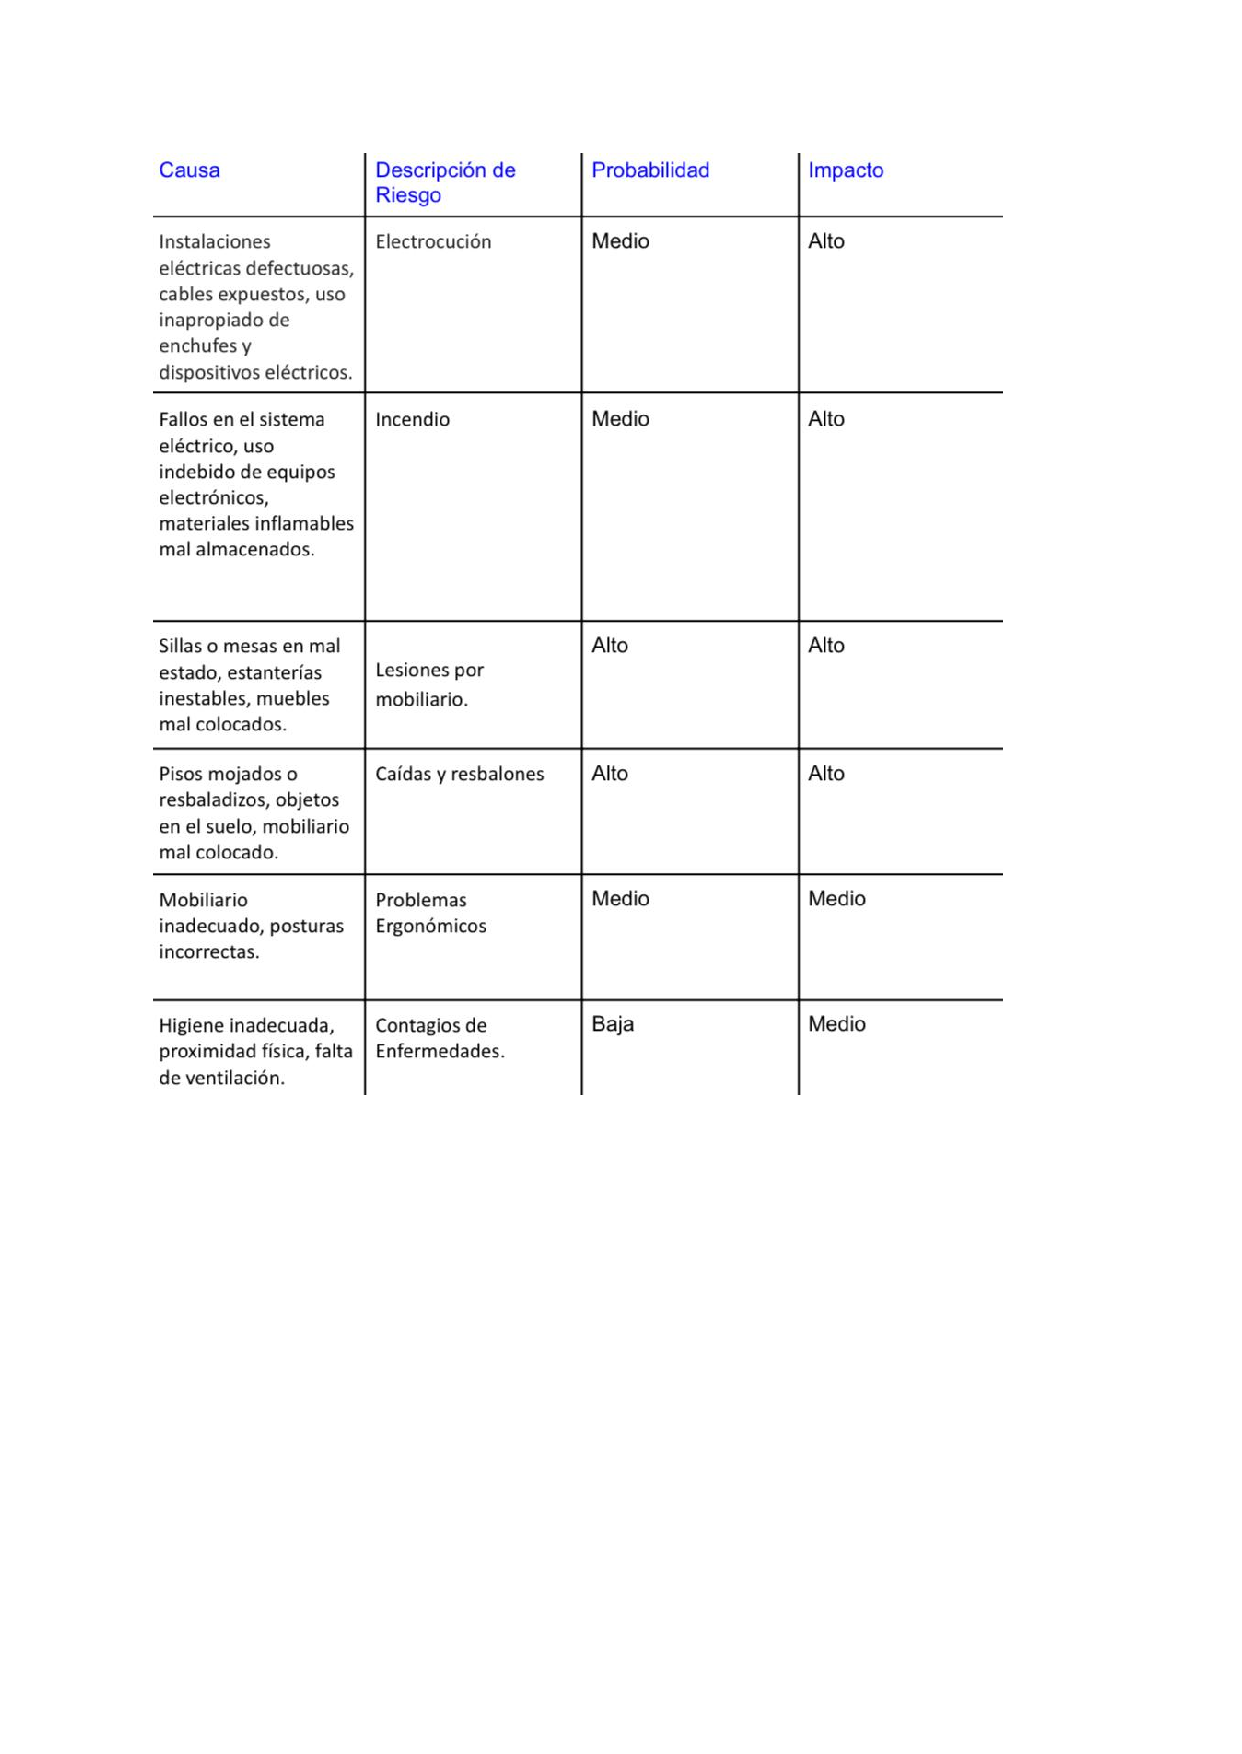
\includegraphics[trim = {0mm 0mm 0mm 0mm},clip,scale=0.3]{20/img/Riesgos Internos.pdf}
        \end{figure}
    A.6. Riesgos Externos:
     Desastres Naturales.
     Emergencias de Salud Pública.
     Riesgos de Seguridad.
     Riesgos Ambientales.
     Problemas de Infraestructura Cercana
    \begin{figure}[H]
        \centering
        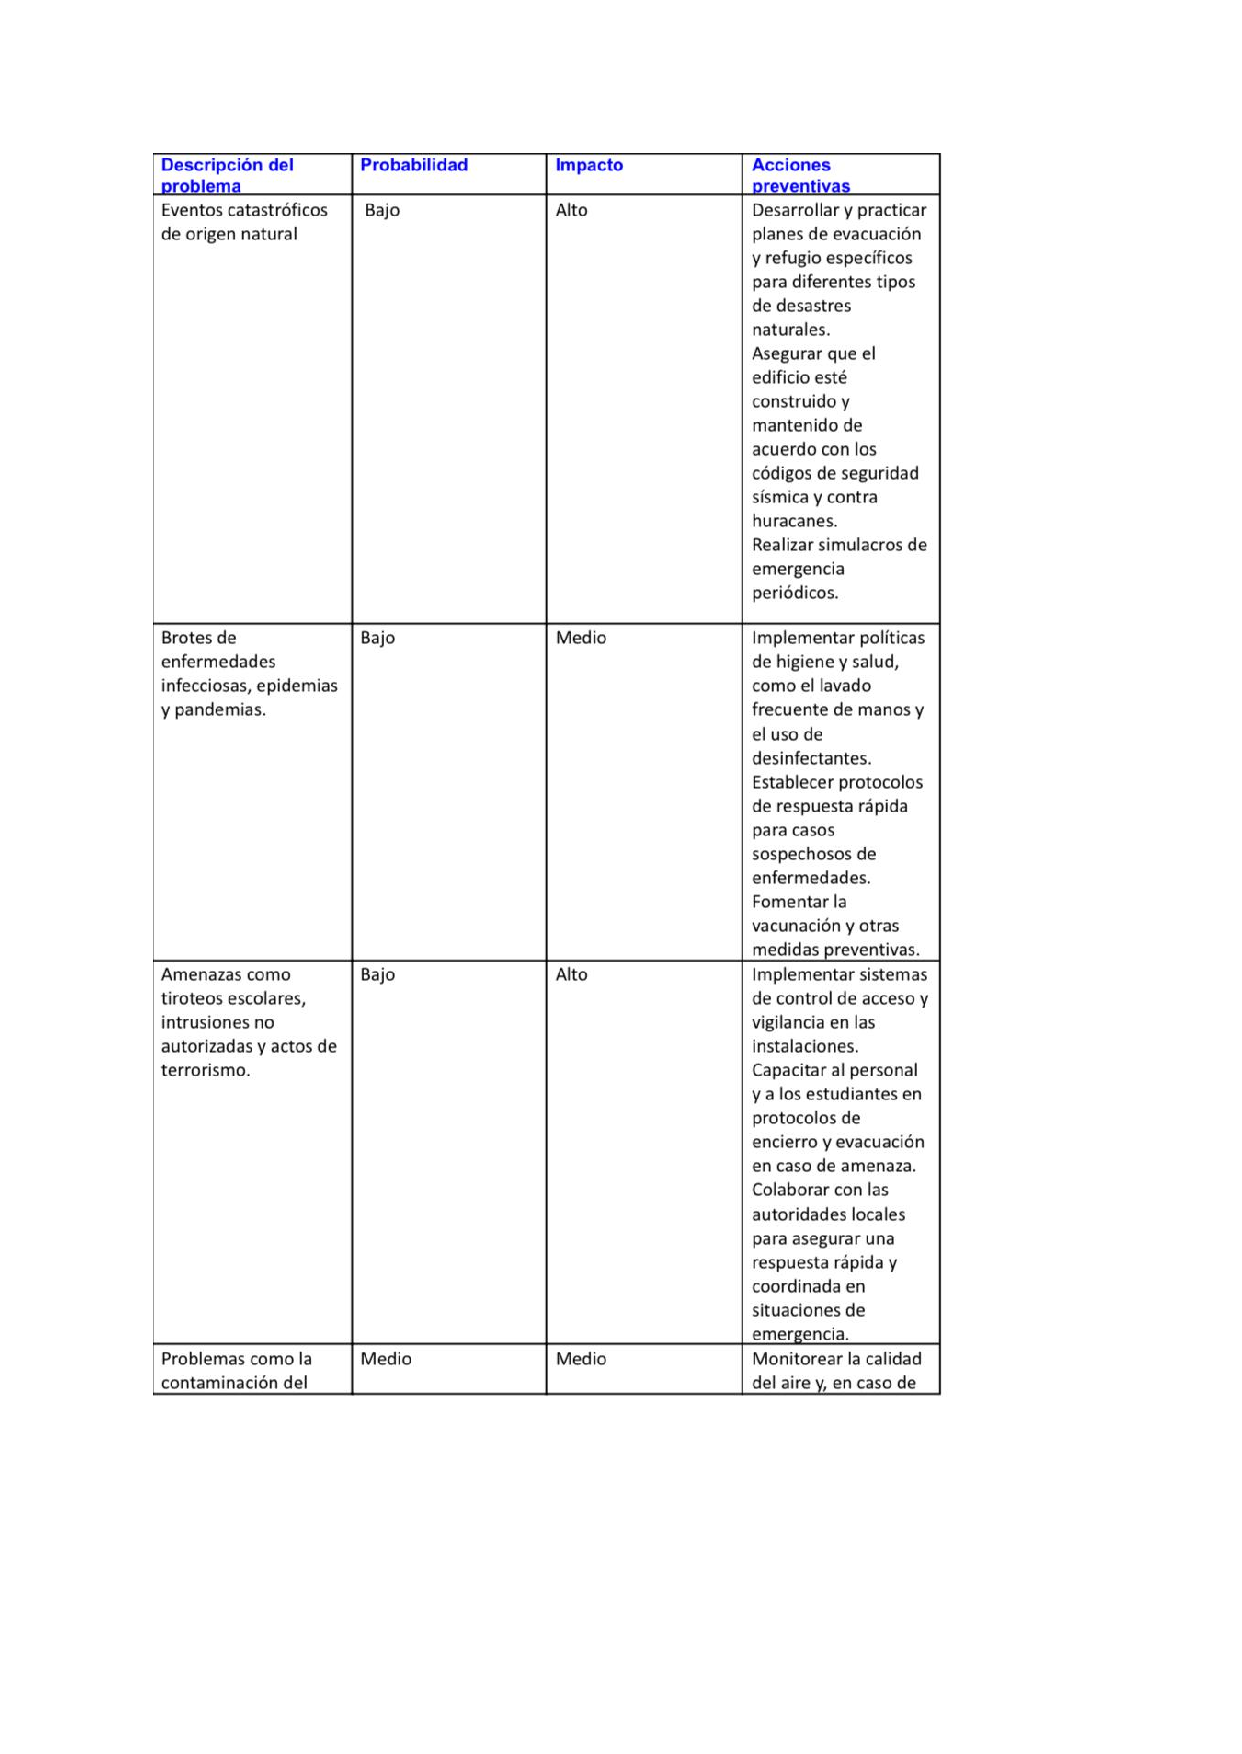
\includegraphics[trim = {0mm 0mm 0mm 0mm},clip,scale=0.4]{20/img/Riesgos Externos.pdf}
        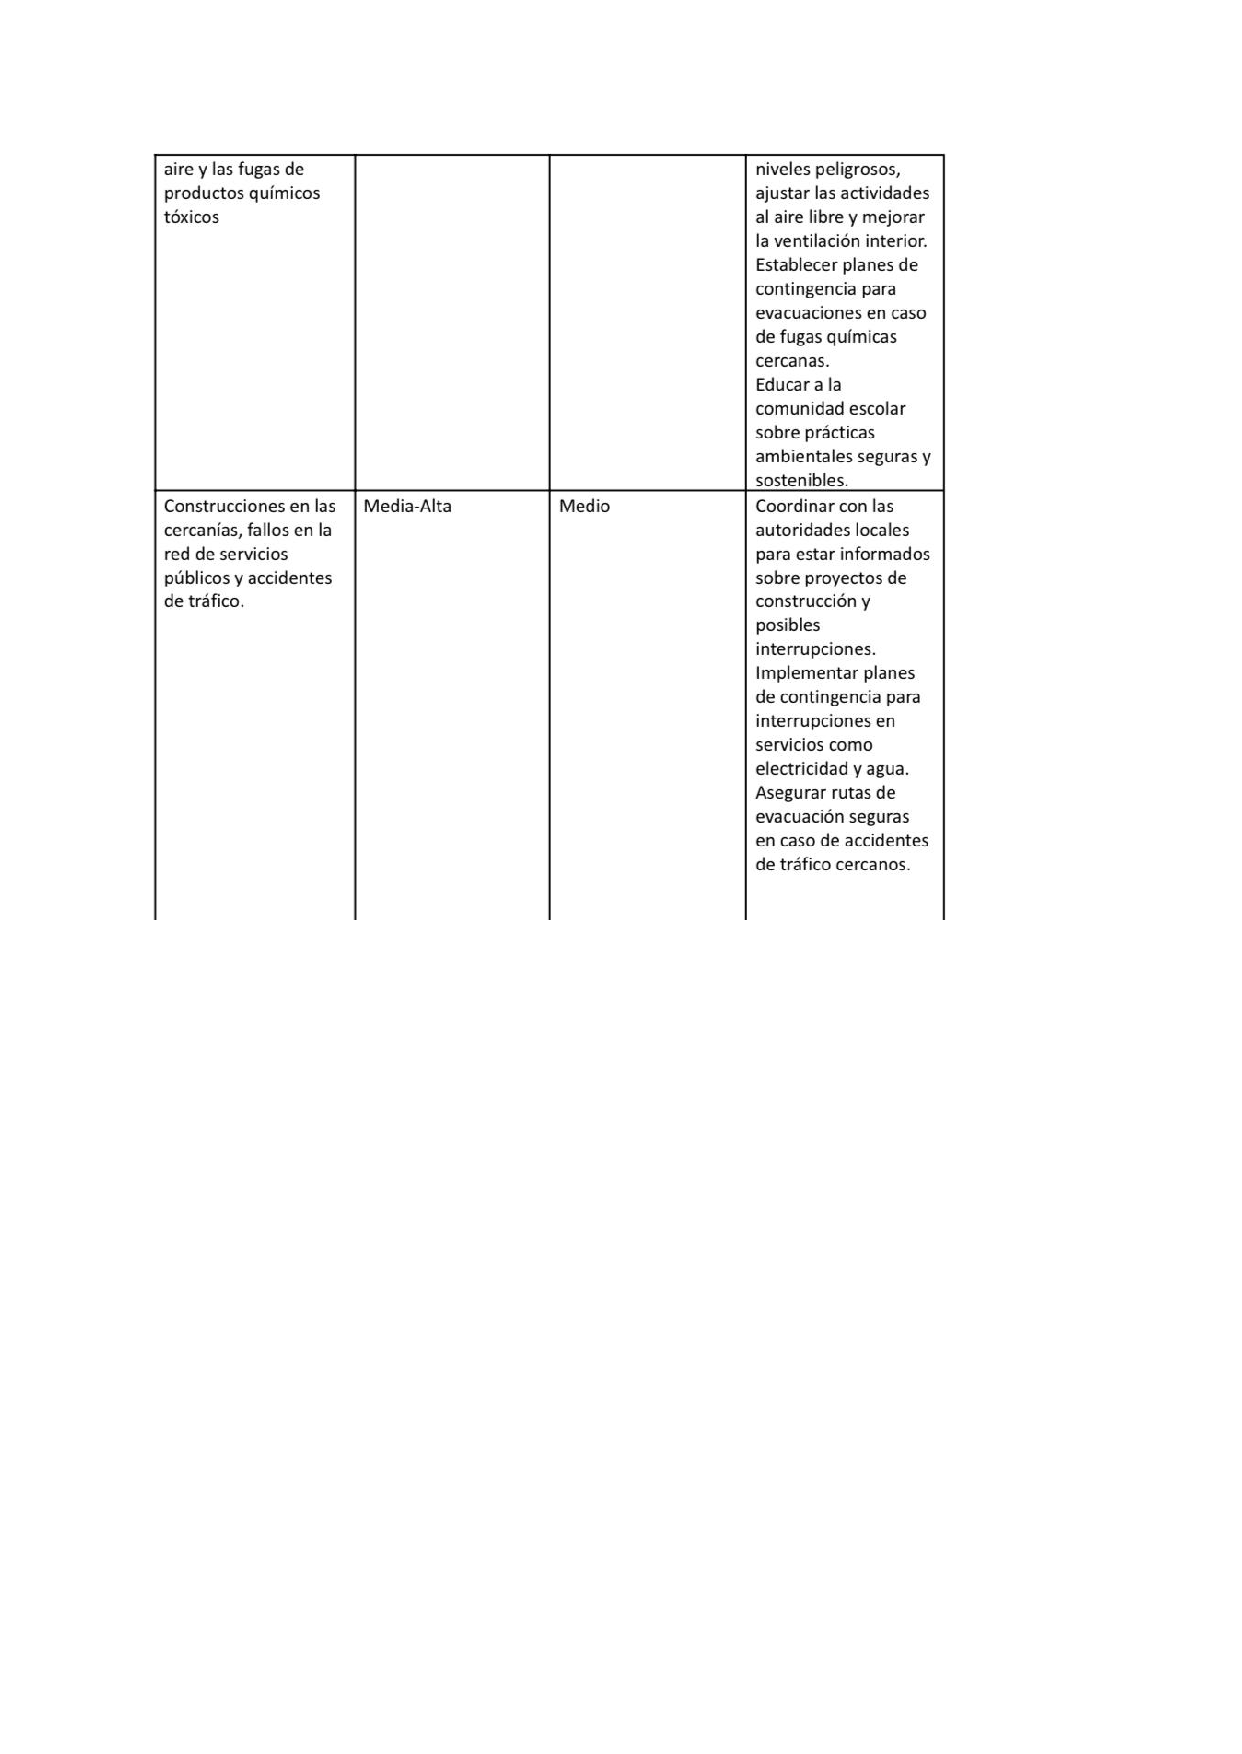
\includegraphics[trim = {0mm 0mm 0mm 0mm},clip,scale=0.4]{20/img/Riesgos Externos2.pdf}
        \end{figure}
    A.7. Y A.8.  Identificación de capacidades
    \begin{figure}[H]
        \centering
        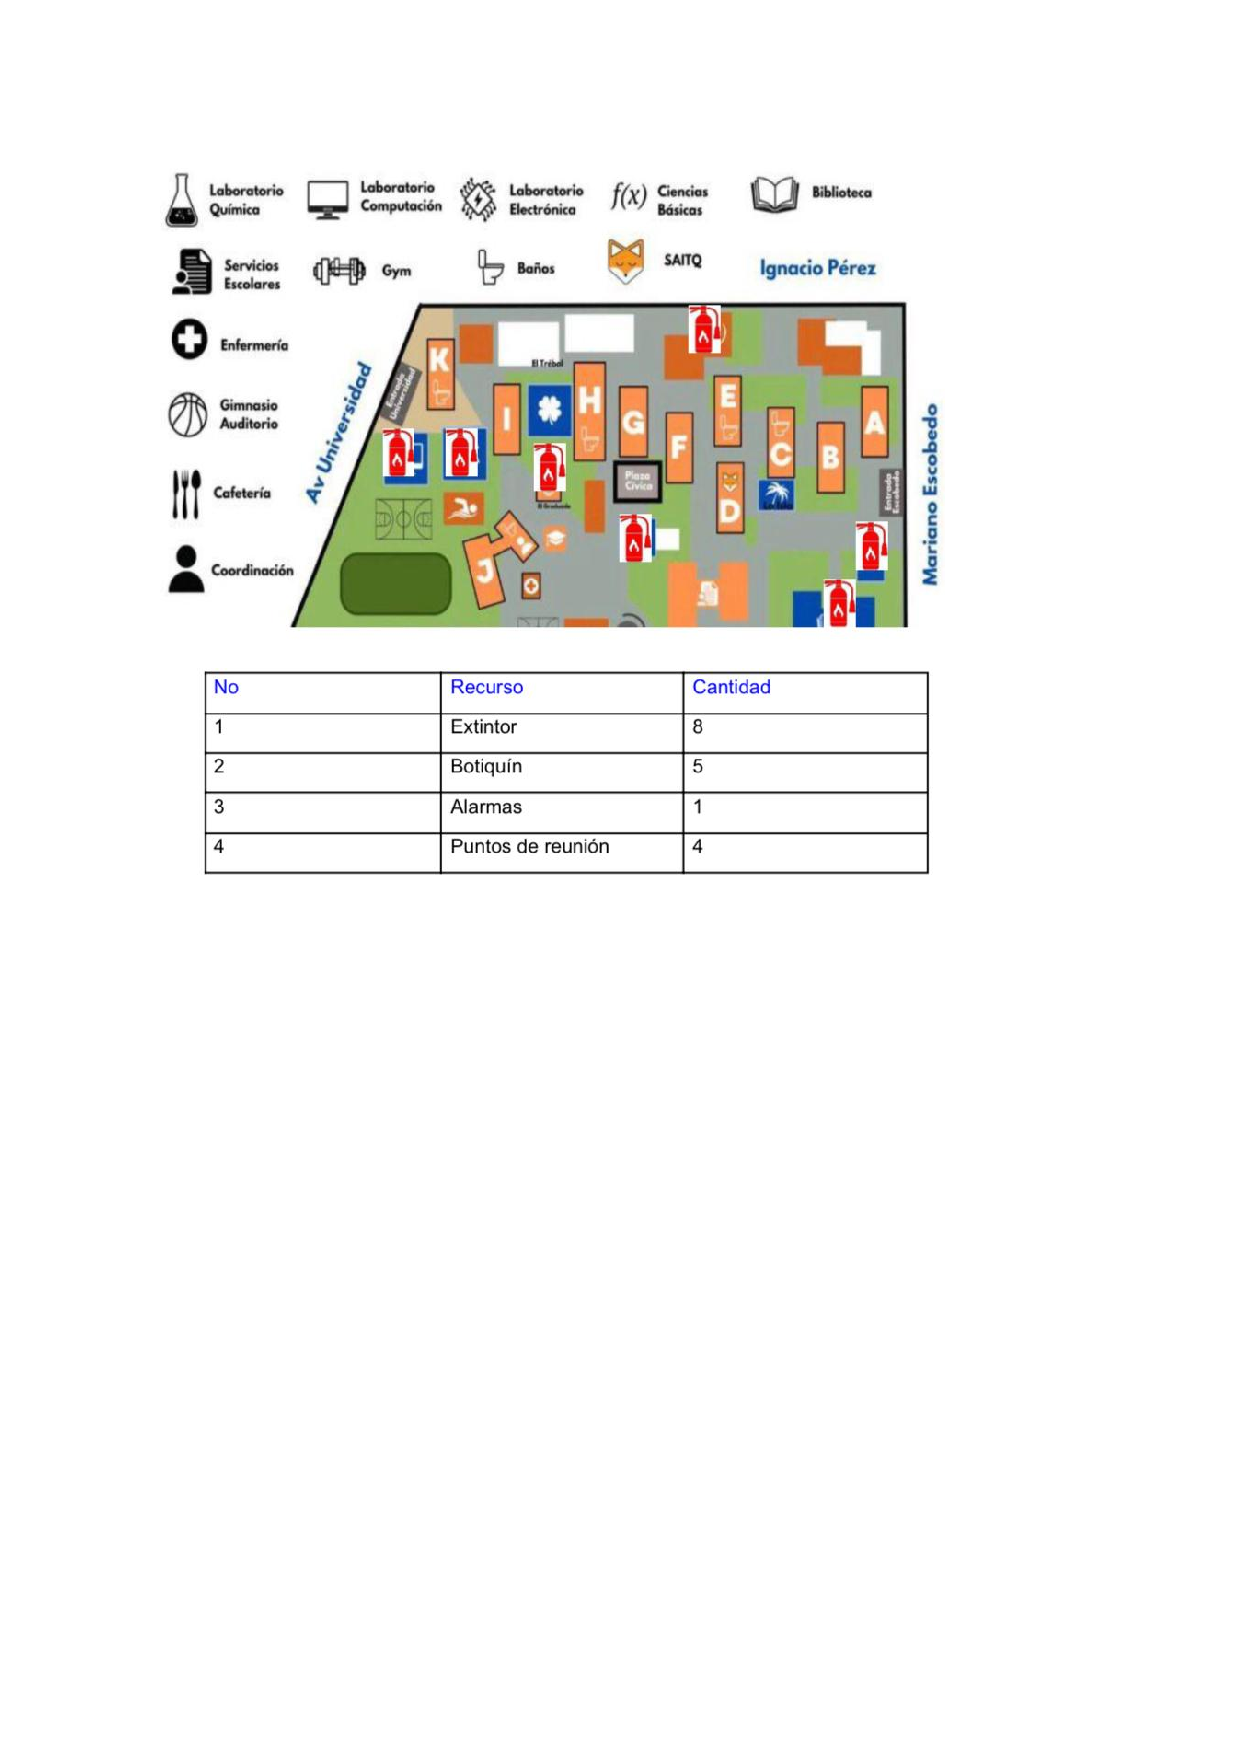
\includegraphics[trim = {0mm 0mm 0mm 0mm},clip,scale=0.3]{20/img/Identificacion de capacidades.pdf}
        \end{figure}
     A.9.  Identificación de apoyos externos:
     ISSSTE Hospital General
    Ofrece servicios de salud integral a afiliados, trabajadores, jubilados y sus familias.
    Dirección: Av. Tecnológico N° 101, Las Campanas, Santiago de Querétaro, Querétaro, México
    Teléfono: 442 215 4944
    Horario:
    Lunes a Sábado 7:00 – 20:00 horas.
    Sala de emergencia las 24 horas.
    Bomberos
    Zaragoza No. 90, 76000 Querétaro, QUERÉTARO
    442 212 1314
    bomberosqueretaro.com
    Horario:Miércoles a domingo: 11:00-19:00 horas.
    Guardia nacional
    136,Calle Estadio, 76090 Centro Sur, Querétaro
    442 428 6600
    Horario: Lunes a Viernes: 8 am- 3 am.
    Secretaría de Seguridad Ciudadana
    Paseo 5 de Febrero No. 35 Norte, Col. San Antonio de la Punta, Qro., C.P. 76010
    Teléfono
    (442) 309 14 00 / (442) 309 14 13
    Mail
    prevención@queretaro.gob.mx
    Lunes a viernes de 08:00 a 18:00 horas en días hábiles.Sábado 08:00 a 12:00 horas atención al
    público.
    
    A.10. Plan de evacuación y repliegue:
    Responsable de Seguridad (Nieves Jimenez Ana Sofia):
    Equipo: Radios de comunicación, chaleco reflectante.
    Acciones:
    Coordinar la evacuación desde el centro de control.
    Dirigir al equipo de evacuación y asegurarse de que los pasillos estén despejados.
    Supervisar el repliegue en caso de una emergencia.
    Encargado de Primeros Auxilios (Ruiz Peña Nancy):
    Equipo: Botiquín de primeros auxilios.
    Acciones:
    Proporcionar primeros auxilios a los heridos durante la evacuación.
    Organizar un punto de reunión seguro para atender a los heridos.
    Coordinar con servicios médicos externos si es necesario.
    Coordinador de Evacuación (Llamas Nuñez Ana Valeria):
    Equipo: Lista de estudiantes y personal, megáfono.
    Acciones:
    Supervisar la evacuación de edificios y dirigir a las personas hacia las salidas de emergencia.
    Asegurar que todos los estudiantes y personal abandonen el edificio de manera ordenada.
    Informar al Responsable de Seguridad sobre el progreso de la evacuación.
    Encargado de Acompañamiento (Fentanez Hernandez Ana Karen):
    Equipo: Identificación de seguridad, lista de verificación de evacuación.
    Acciones:
    Ayudar a los estudiantes con necesidades especiales a evacuar de manera segura.
    Acompañar a los grupos de estudiantes hasta el punto de reunión designado.
    Comprobar que todos los estudiantes y personal hayan sido evacuados.
    Coordinador de Repliegue (Sanchez Hernandez Edwin Ernesto):
    Equipo: Plan de repliegue, mapa de rutas de escape.
    Acciones:
    Evaluar la situación y decidir si es necesario un repliegue en caso de emergencia.
    Coordinar la retirada ordenada de las personas hacia áreas seguras en caso de amenaza externa.
    Mantener comunicación con el Responsable de Seguridad para recibir instrucciones adicionales.
    
    Procedimiento de Evacuación y Repliegue
    Anuncio de Emergencia:
    El Responsable de Seguridad activará la alarma de emergencia y anunciará la situación a través de los
    altavoces del campus.
    Evacuación Ordenada:
    El Coordinador de Evacuación y su equipo dirigirán a estudiantes y personal hacia las salidas de
    emergencia más cercanas.
    Asistencia a Personas con Necesidades Especiales:
    El Encargado de Acompañamiento proporcionará apoyo adicional a personas con discapacidades o
    necesidades especiales durante la evacuación.
    Atención Médica de Emergencia:
    El Encargado de Primeros Auxilios proporcionará asistencia médica básica a los heridos en un área
    segura.
    Reunión en Punto Designado:
    Todos los grupos de evacuación se reunirán en un punto designado fuera del edificio para realizar un
    conteo y asegurarse de que todos estén presentes.
    Comunicación y Actualización:
    El Coordinador de Evacuación mantendrá informado al Responsable de Seguridad sobre el progreso
    de la evacuación y cualquier problema encontrado.
    Repliegue en Caso de Amenaza Externa:
    En caso de una amenaza externa, como un tiroteo cerca del campus, el Coordinador de Repliegue
    evaluará la situación y coordinará el repliegue hacia áreas seguras.
    Regreso al Edificio:
    El Responsable de Seguridad autorizará el regreso al edificio una vez que se haya determinado que es
    seguro hacerlo.
    Este plan de evacuación y repliegue proporciona un marco claro de acción para el personal
    designado en caso de una emergencia en la universidad, garantizando una respuesta rápida y
    efectiva para proteger la seguridad y el bienestar de todos los estudiantes y el personal.
    
    % 
    % 
    \subsection{Análisis de los métodos, materiales, herramientas e instalación utilizada en la ejecución del ensamble de un circuito electrónico}
    
    \subsubsection{Planeación}
    
    % 
    % 
    \subsubsection{5's}
    
    La metodología de las 5S es una herramienta de gestión japonesa que busca mejorar la organización, limpieza y eficiencia en el lugar de trabajo.
    1. Seiri (Clasificación/Separación):
    
    Eliminar todo lo que no sea necesario en la mesa de trabajo. Retira herramientas, documentos o suministros que no se utilicen con frecuencia.
    Clasificar los elementos restantes en categorías, como herramientas, materiales, documentos, etc.
    Decidir qué elementos son esenciales y cuáles pueden ser almacenados en otro lugar.
    2. Seiton (Orden):
    
    Organizar los elementos restantes de manera ordenada y accesible en la mesa de trabajo.
    Utilizar cajas, estanterías, soportes u otros dispositivos de almacenamiento para mantener las herramientas y materiales en su lugar.
    Etiquetar los elementos o utiliza marcadores para identificar claramente dónde va cada cosa.
    3. Seiso (Limpieza):
    
    Limpiar la mesa de trabajo a fondo, eliminando el polvo, residuos o cualquier otro tipo de suciedad.
    Establecer un programa regular de limpieza para mantener la mesa de trabajo limpia y ordenada en todo momento.
    Fomentar la cultura de la limpieza entre todos los empleados que utilizan la mesa de trabajo.
    4. Seiketsu (Estandarización):
    
    Establecer estándares claros para el mantenimiento de la mesa de trabajo. Definir cómo deben organizarse los elementos, qué nivel de limpieza se espera y quién es responsable de mantenerlo.
    Crea listas de verificación o procedimientos estandarizados para el uso y la limpieza de la mesa de trabajo.
    Capacitar al operador sobre los estándares y la importancia de mantener la mesa de trabajo en condiciones óptimas.
    5. Shitsuke (Disciplina):
    
    Fomentar una cultura de responsabilidad y disciplina entre el operador para seguir los estándares establecidos.
    Realizar auditorías regulares para verificar el cumplimiento de los estándares y brindar retroalimentación al operador.
    Reconocer y premiar el cumplimiento y el mantenimiento de los estándares de las 5S en la mesa de trabajo.
    % 
    % 
    \subsubsection{Desarrollo del sistema de tiempos predeterminado}
    % 
    % 
    
    \subsubsection{Desarrollo del muestreo del trabajo}
    % 
    % 
    
    \subsubsection{Corrección por balanceo de procesos}
    % 
    % 
    
    \subsubsection{Datos estándar continuos y discretos}
    % 
    % 
    
    \begin{itemize}
        \item Se debe establecer que se habrá de hacer, como, conque, y donde para obtener la información que permita probar la hipótesis.  
        \item Se debe desglosar de acuerdo a los objetivos específicos. 
        \item Se debe establecer una estrategia metodológica por cada objetivo específico. De manera simplista se podría decir que se cambia el verbo en infinitivo por su respectivo adverbio.
        \item En cada objetivo se debe describir que método, que materiales y que equipo se usará para conseguirlo.
    \end{itemize}
    %
    % 
    
    \subsection{Prepara tu documento}
    
    Antes de que comiences a utilizar esta plantilla, es recomendable que prepare la información que contendrá en un archivo aparte. 
    Ten preparadas tus gráficas, así como también las tablas aparte, para que sea más fácil integrarlo. 
    Se recomienda fuertemente el uso de \textbf{formato Enhanced Metafile (.emf) para imágenes y gráficas} de resolución óptima. 
    Finalmente, completa y organiza el contenido antes de darle el formato de esta plantilla. 
    
    \subsection{Acrónimos y Abreviaciones}
    
    Los acrónimos y abreviaciones deberán ser definidos únicamente la primera vez que aparecen en el texto, esto para que el lector entienda lo que significan.
    
    \subsection{Ecuaciones}
    
    Las ecuaciones son una excepción a las especificaciones prescritas de esta plantilla. 
    Deberá determinar si su ecuación debe escribirse o no utilizando la fuente Adobe Devangari. 
    Para crear ecuaciones multinivel, puede ser necesario tratar la ecuación como un gráfico e insertarla en el texto después de aplicar el estilo de la platilla.
    Las ecuaciones serán enumeradas de manera consecutiva, y el número de ecuación, entre paréntesis, se colocan al ras de la derecha, utilizando una tabulación derecha. 
    
    \begin{equation}
        \label{eq1}
        x + y = z 
    \end{equation}
    
    Es importante asegurarse de que los símbolos de la ecuación sean definidos antes o inmediatamente después de la ecuación. Utilice “(1)”, en vez de “Eq. 1” al enumerar las ecuaciones, excepto al principio de una oración: “La ecuación (\ref{eq1}) es…”
    
    \section{Resultados y discusión}
    
    En base a la metodología presentada se elaboró la conexión del circuito con Arduino.
    \begin{figure}[H]
        \centering
        \includegraphics[trim = {0mm 0mm 0mm 0mm},clip,scale=0.3]{20/img/Evidencia del circuito armado .pdf}
        \caption{Evidencia1}
        \end{figure}
        \begin{figure}[H]
         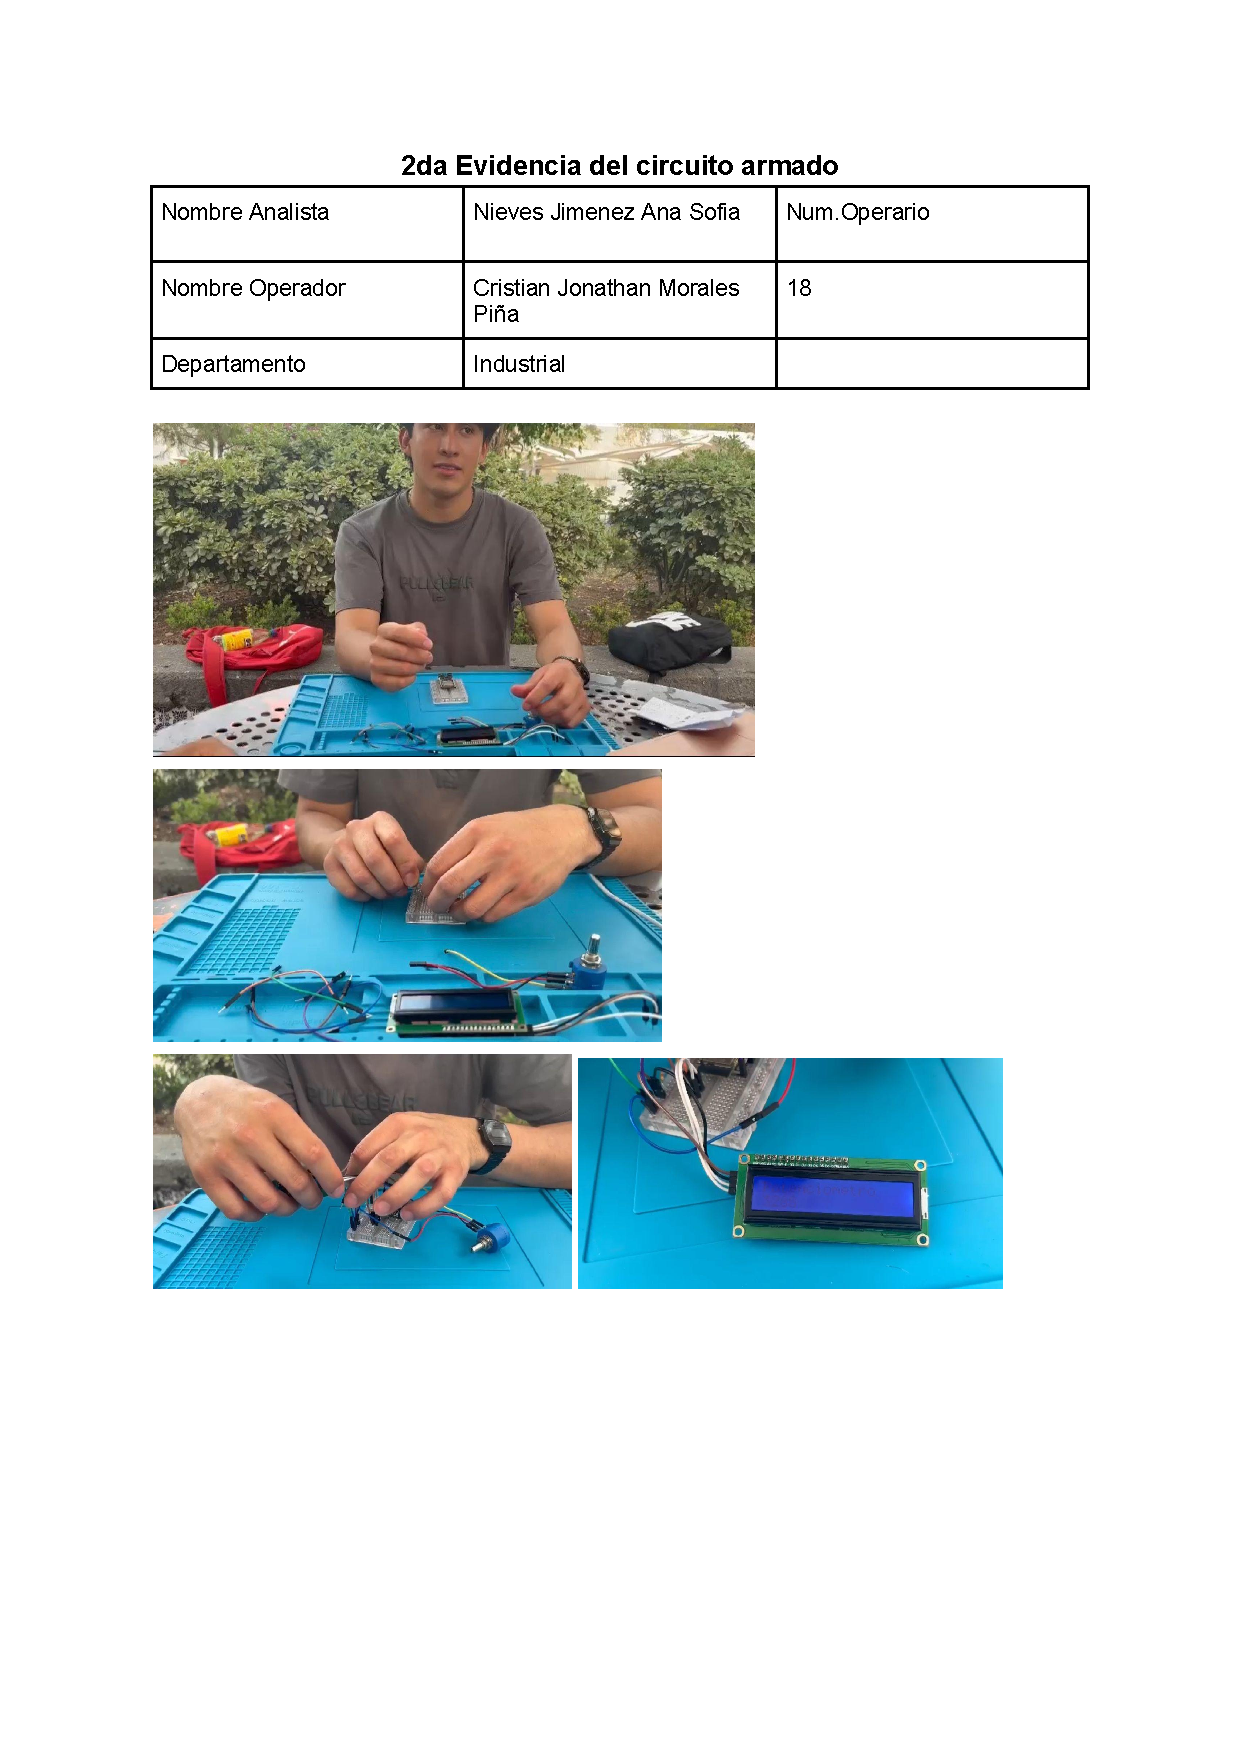
\includegraphics[trim = {0mm 0mm 0mm 0mm},clip,scale=0.3]{20/img/2da Evidencia del circuito armado.pdf}
        \caption{Evidencia2}
    \end{figure}
    
    \begin{figure}[H]
        \centering
        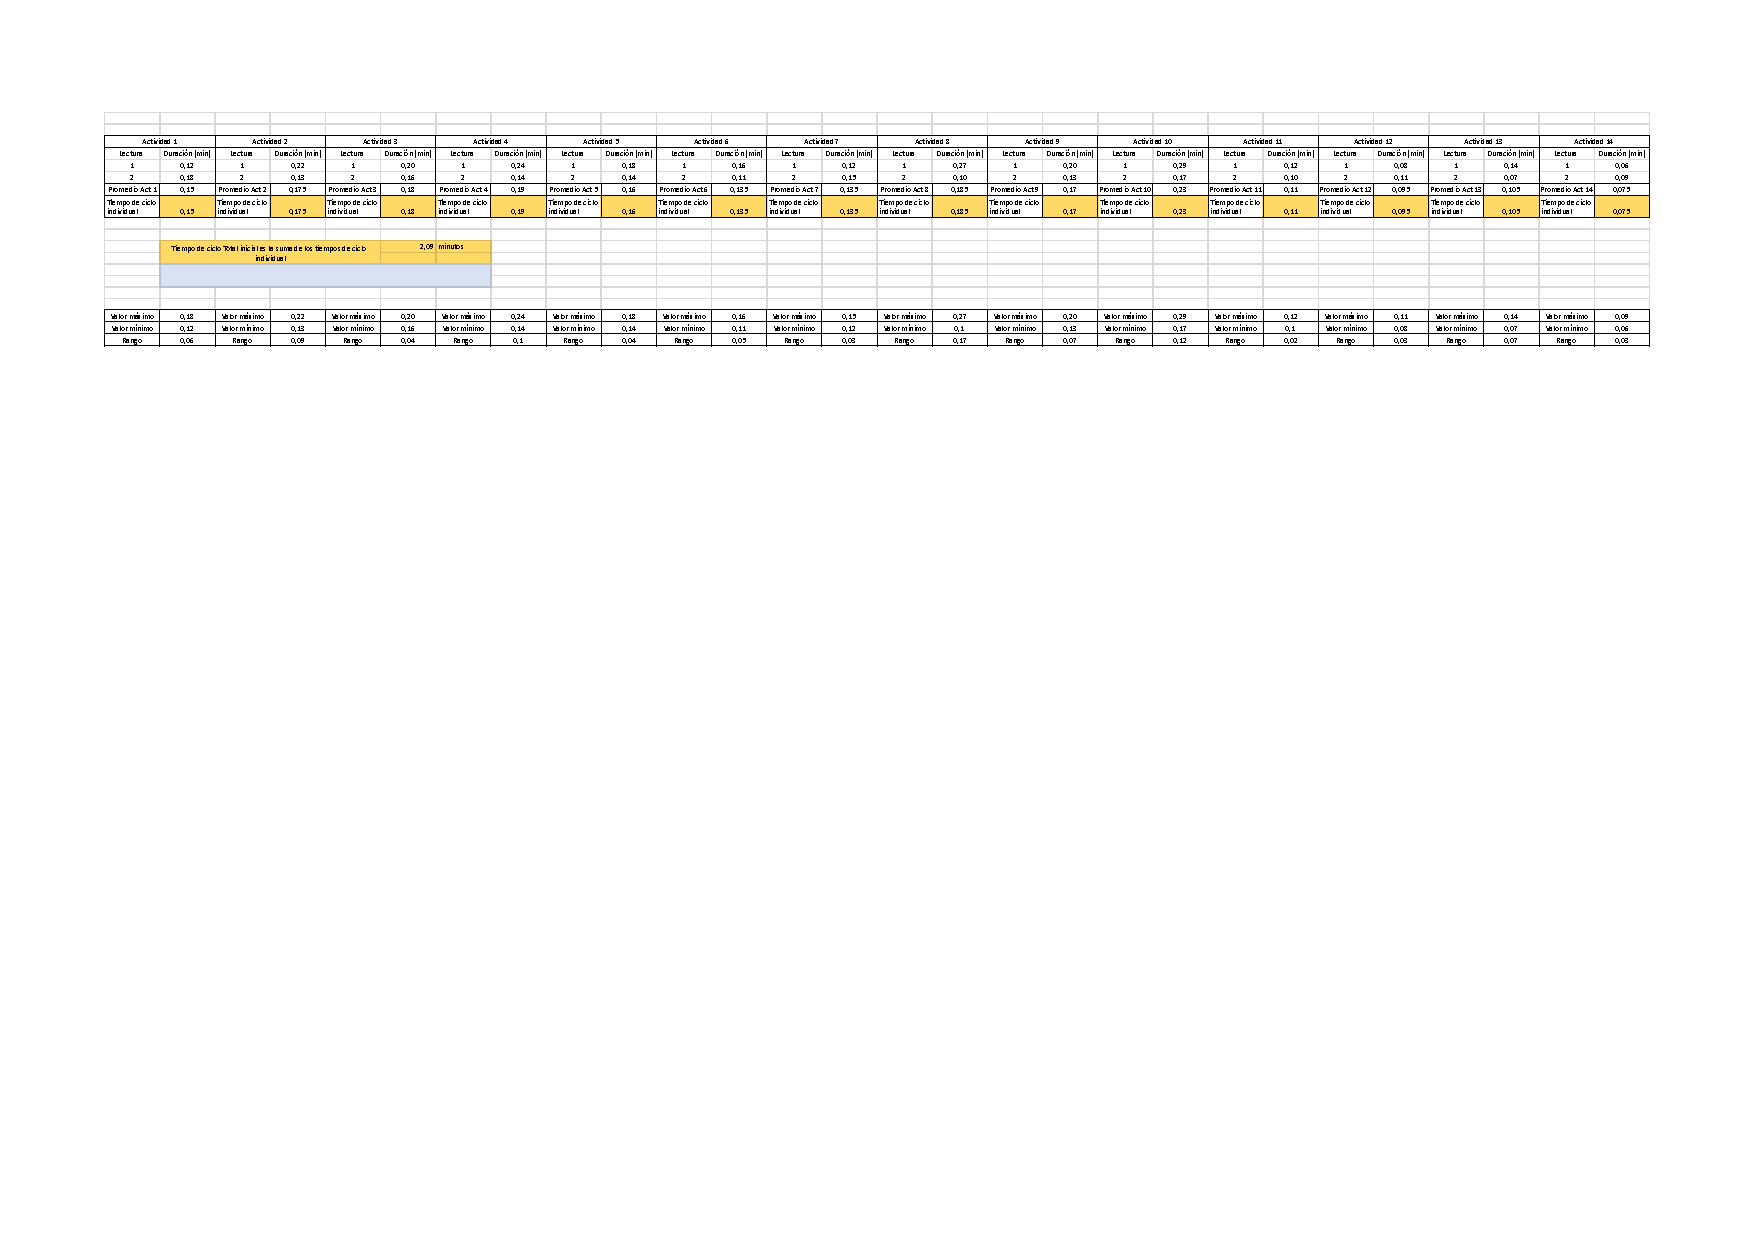
\includegraphics[trim = {0mm 0mm 0mm 0mm},clip,scale=0.3
        ]{20/img/Tiempo Ciclo Ensamble - Hoja 1.pdf}
        \caption{Tiempo Ciclo}
        \end{figure}
    
    \subsection{Autores y Afiliaciones}
    
    Para distinguir las afiliaciones de los autores, utilice superíndices iniciando con el número 1, 2, etc., sucesivamente, esto dependerá de la cantidad de los departamentos a los que estén afiliados los autores. En caso de que todos los autores pertenezcan a una mismo departamento e institución, utilizar sólo el superíndice 1. 
    
    \subsection{Identificar los encabezados}
    
    Se les recuerda a los autores que los encabezados deben de estar conforme los solicita la guía del autor. De ahí se puede adaptar el trabajo para que sea más fácil de entender para el lector.
    Los encabezados organizan los temas sobre una base relacional y jerárquica. Por ejemplo, el título del documento es encabezado del texto principal porque todo el material posterior se relaciona y elabora sobre este tema. 
    
    \subsection{Tablas y Figuras}
    
    \begin{enumerate}
        \item Posición de las tablas y figuras: Coloque las figuras y las tablas en la parte superior e inferior de las columnas. Evite colocarlos en medio. Las figuras y las tablas grandes pueden abarcar ambas columnas. Los títulos de las figuras deben de estar debajo de las mismas; los títulos de las tablas deben aparecer encima de ellas. Insértese las figuras y los cuadros después de citarse en el texto. Utilice la abreviatura “Fig. 1”, incluso al principio de una oración. 
    \end{enumerate}
    
    \section{Conclusiones}
    
    Se describe aquí el alcance del trabajo, logros obtenidos y perspectivas para el futuro de este. Se sugiere colocar información cuantitativa obtenida.
    
    \section{Agradecimientos}
    
    Es importante darles su debido reconocimiento a los laboratorios, instituciones, organizaciones, entre otros que han sido participes para la culminación de este trabajo. También es importante mencionar, fondos, proyectos, becas, entre otros que se le han otorgado al o los autores para realizar el trabajo de investigación. Ejemplo: “Los autores agradecen al Concejo Nacional de Ciencia y Tecnología por los recursos otorgados…”
    
    \section*{Referencias}
    
    
    % Ejemplo
    %  @Article{article,
    % 	author = "Author1 LastName1 and Author2 LastName2 and Author3 LastName3",
    % 	title = "Article Title",
    % 	volume = "30",
    % 	number = "30",
    % 	pages = "10127-10134",
    % 	year = "2013",
    % 	doi = "10.3389/fnins.2013.12345",
    % 	URL = "http://www.frontiersin.org/Journal/10.3389/fnins.2013.12345/abstract",
    % 	journal = "Frontiers in Neuroscience"
    % }
    
    % @book{book,
    %   author    = {Author Name}, 
    %   title     = {The title of the work},
    %   publisher = {The name of the publisher},
    %   address   = {The city},
    %   year      = 1993,
    % }
    
    % @incollection{chapter,
    %   author       = {Bauthor Surname}, 
    %   title        = {The title of the work},
    %   editor       = {Editor Name},
    %   booktitle    = {The title of the book},
    %   publisher    = {The name of the publisher},
    %   address      = {The city},
    %   year         = 2002,
    %   pages        = {201-213},
    % }
    
    % @InProceedings{conference,
    %   author = {Cauthor Name and Dauthor Surname and Fauthor LastName},
    %   title = {The title of the work},
    %   booktitle = {The title of the conference proceedings},
    %   year = 1996,
    %   publisher = {The name of the publisher},
    %   editor = {Editor Name1 and Editor Name2},
    %   pages = {41-50},
    % }
    
    % @book{cho,
    %   author       = {Gauthor Name1}, 
    %   title        = {The title of the work},
    %   publisher = {Country code and patent number},
    %   address      = {Patent Country},
    %   year = 2013
    % }
    
    % @book{patent,
    %   author    = {Hauthor Surname1}, 
    %   title     = {The title of the work},
    %   publisher = {Patent number},
    %   address   = {Patent country},
    %   year      = 2010,
    % }
    
    % % please use misc for datasets
    % @misc{dataset, 
    % 	author = "Author1 LastName1 and Author2 LastName2 and Author3 LastName3",
    % 	title = "Data Title",
    % 	year = "2011",
    % 	doi = "10.000/55555",
    % 	URL = "http://www.frontiersin.org/",
    % }
    
    \bibliographystyle{ieeetr}
    \bibliography{20/referencias
    }
    % 
    % 
    %%%%%%%%%%%%%%%%%%%%%%%%%%%%%%%%%%
    \appendix
    %%%%%%%%%%%%%%%%%%%%%%%%%%%%%%%%%%
    % 
    % 
    \centering{\section[\appendixautorefname{}]{Apéndice}}\label{anexo:pines}
    \includepdf[pages=-]{20/img/Metodología.pdf}
    
    %%%%%%%%%%%%%%%%%%%%%%%%%%%%%%%%%%%%%%%%